%!TEX root = ../PhDThesis.tex



% *********************************************************************************************************************
\chapter{Additional information about the second study}\label{app:studyinfo-cafe}
% *********************************************************************************************************************



This appendix includes additional material to the second study of \acf{VUI} use in a caf\'e (see \autoref{ch:empirical cafe}):

\begin{itemize}
    \item \appref{app:studyinfo-cafe infoconsent} provides the information sheet and consent form given to participants prior to the study,
    \item \appref{app:studyinfo-cafe interview} provides the post-observation interview questions, and
    \item \appref{app:studyinfo-cafe questionnaire} provides the post-observation questionnaire.
\end{itemize}

Additional material related to the study is available on the accompanying CD and online repository:

\begin{itemize}
    \item The descriptive results from the questionnaire are provided in \texttt{studytwo/questionnaire.pdf}.
\end{itemize}



% *********************************************************************************************************************



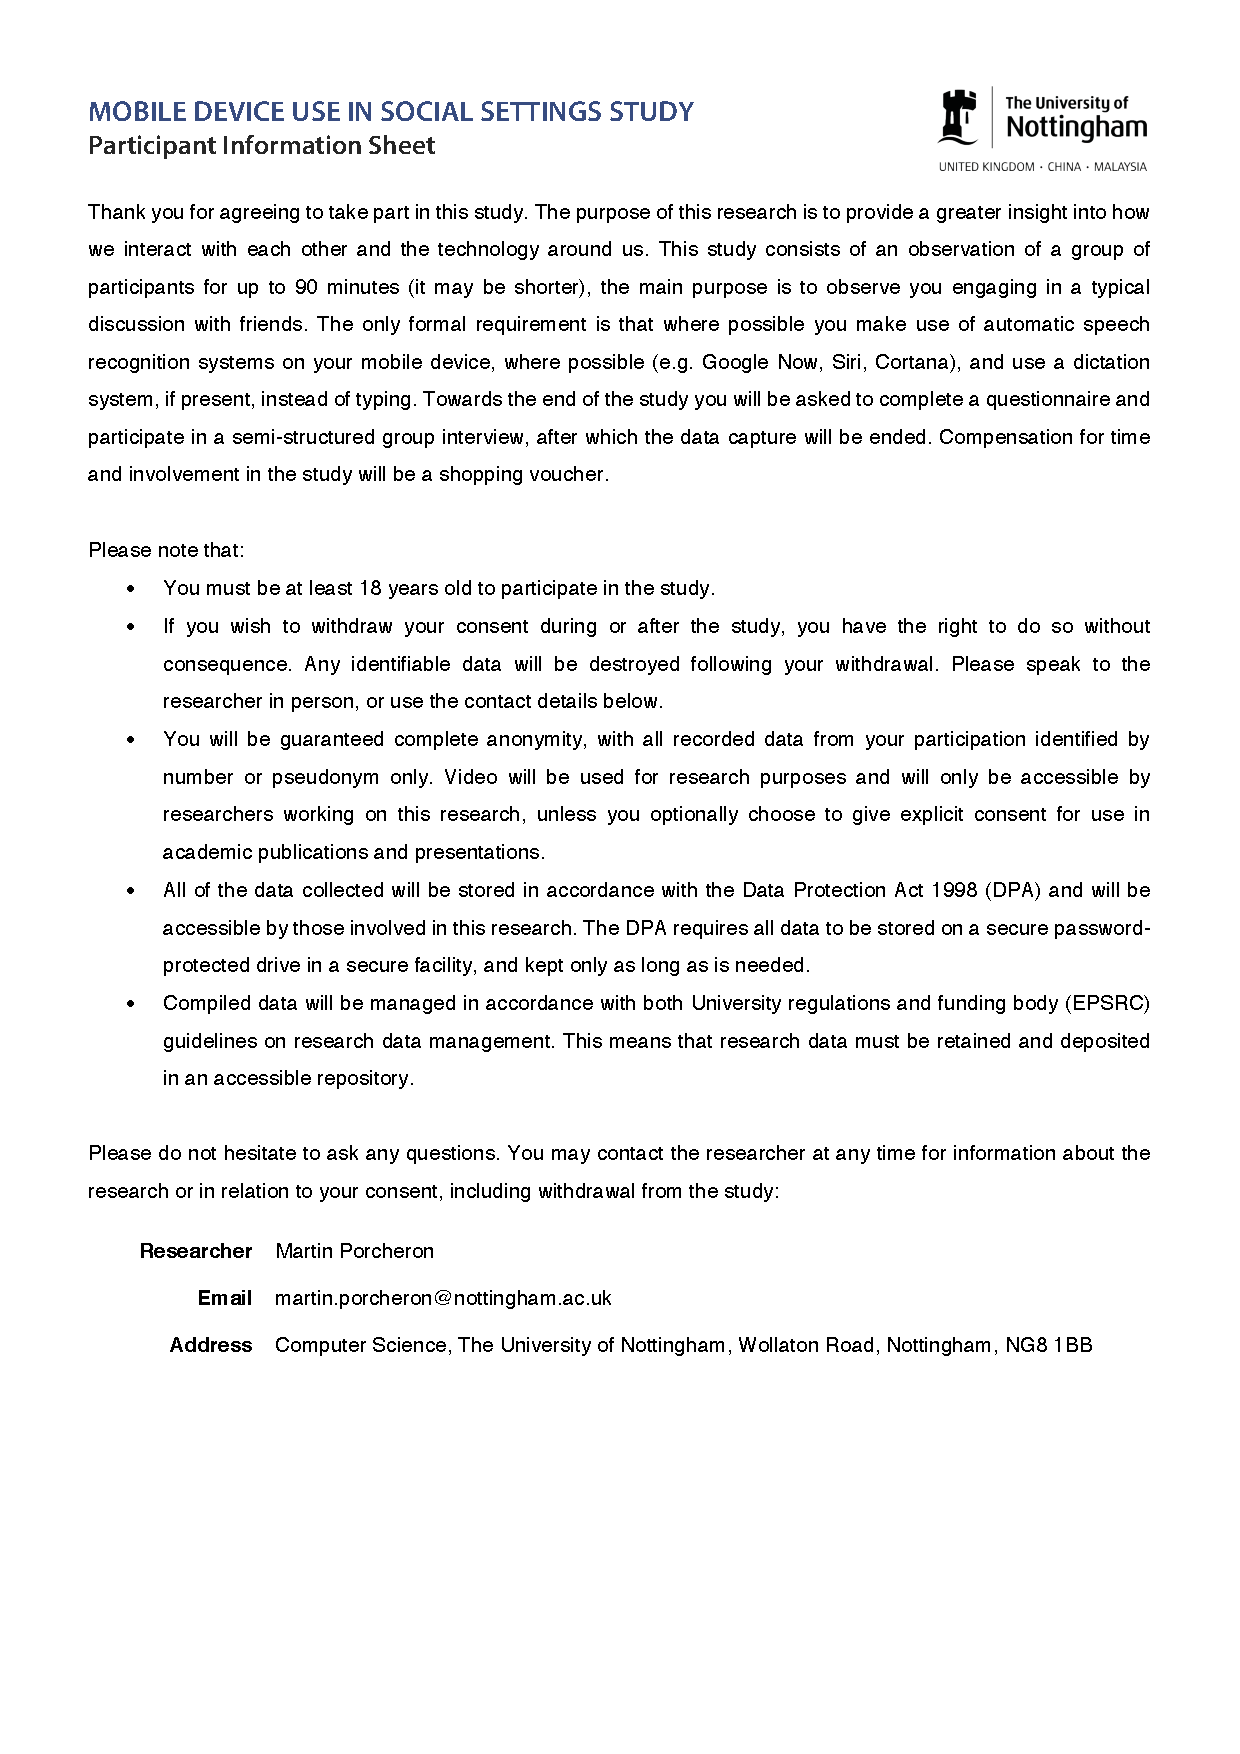
\includepdf[
    pages={1},
    scale=.6,
    frame=false,
    clip,
    trim=1.5cm 1.5cm 1.5cm 1.5cm,
    %offset=-1.05cm 0cm,
    pagecommand={\section{Information sheet and consent form}\label{app:studyinfo-cafe infoconsent}}]
    {Graphics/C-StudyInfo-Cafe/InfoConsent.pdf}
 \includepdf[
    pages={2},
    scale=.6,
    frame=false,
    clip,
    trim=1.5cm 1.5cm 1.5cm 1.5cm,
    %offset=-1.05cm 0cm,
    pagecommand={\nopagebreak}]
    {Graphics/C-StudyInfo-Cafe/InfoConsent.pdf}



% *********************************************************************************************************************



\section{Exit interview questions}\label{app:studyinfo-cafe interview}

\begin{itemize}
    \item How do you feel about the presence of phones in social settings?
    \item Would you say the presence of devices has an impact on the conversation?
    \item Do you recall a time when you have felt ignored by someone using their phone?
    \item How feel about devices attempting to stop you using them at inopportune moments?
    \item Do you see any merits in devices attempting to restrict usage?
    \item Do you feel that people have a responsibility to the group dynamic?
    \item Would you categorise mobiles as a support tool or a distraction device?
    \item Could you see mobile phones being used in conversation without detracting from it?
    \item Would you be willing to take part in further studies that required the installation of an app?
    \item Were you disturbed by presence of cameras or recording equipment?
    \item Did you feel you acted unnaturally due to nature of study?
    \item Did you remain aware of the presence of cameras?
\end{itemize}



% *********************************************************************************************************************



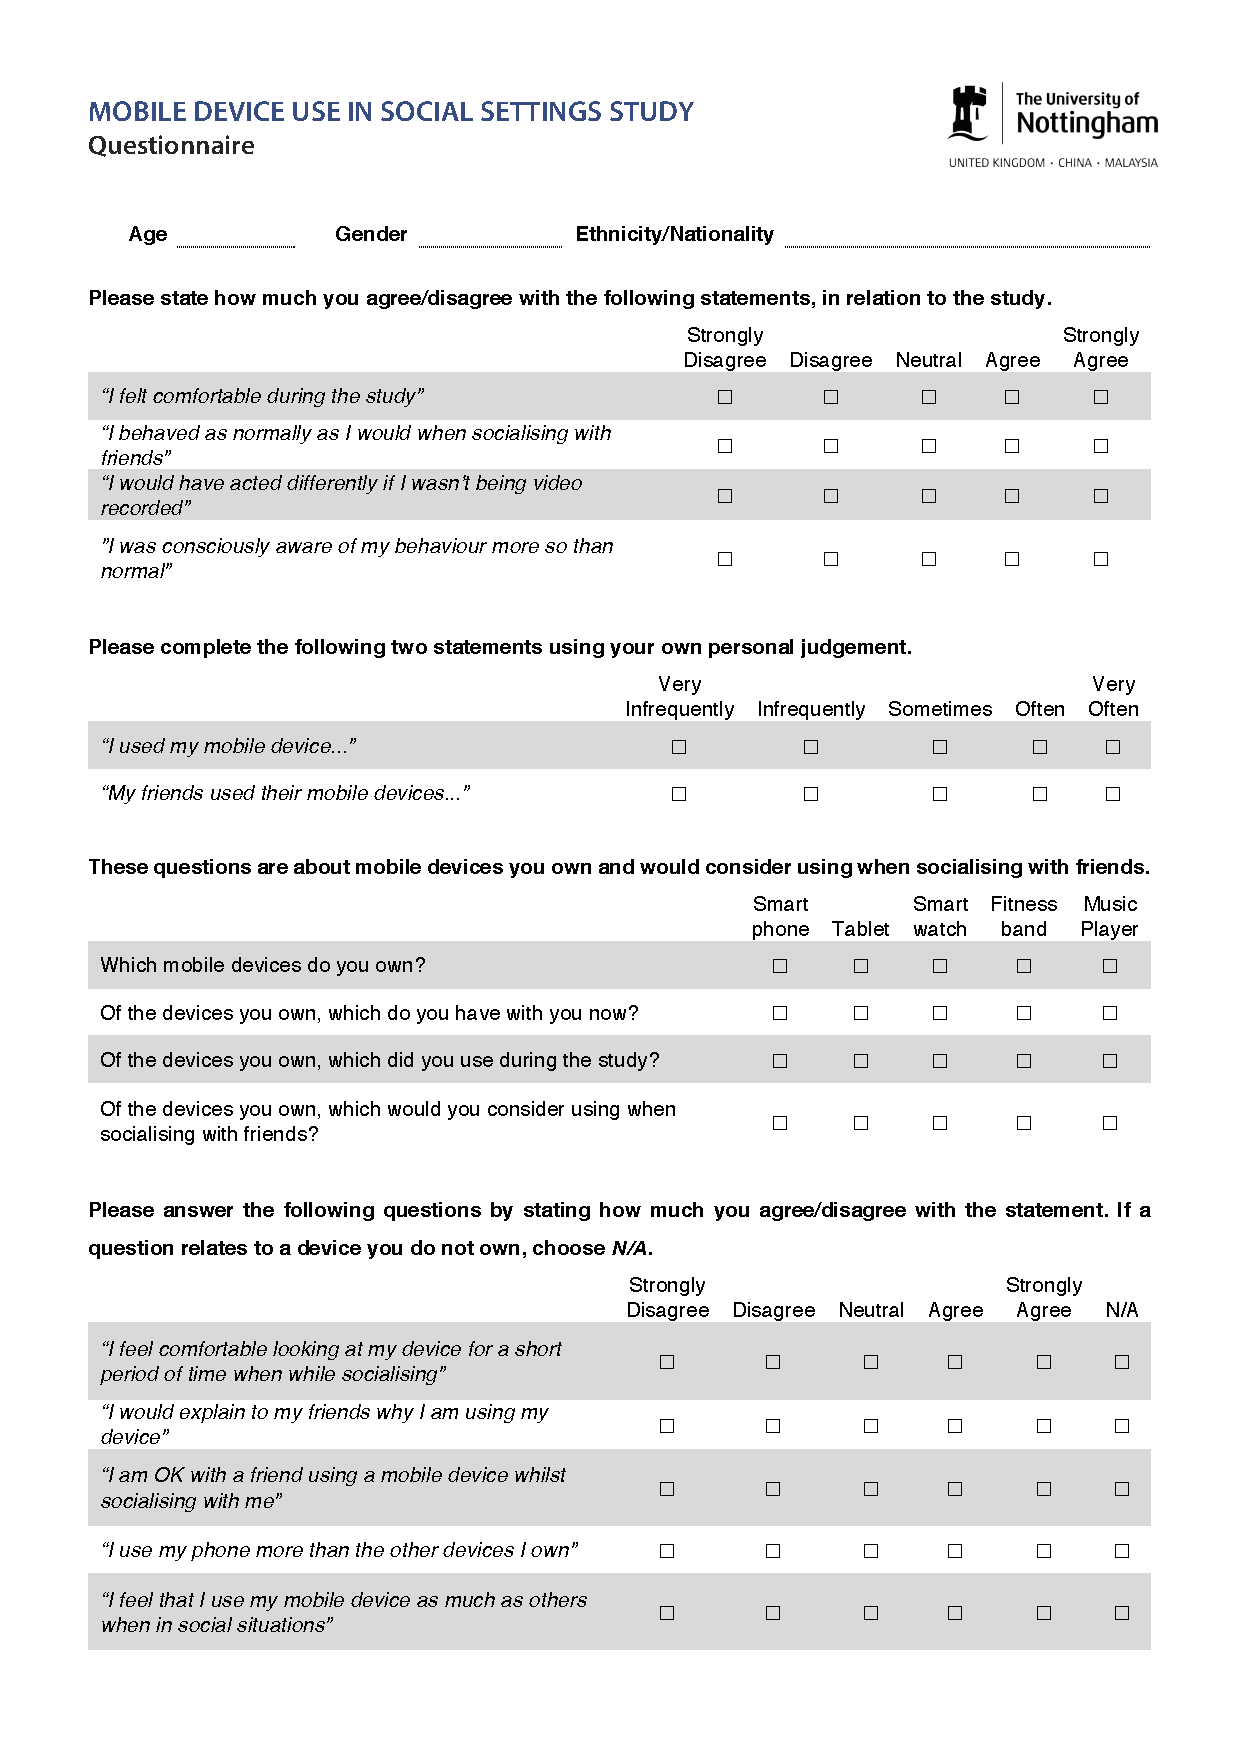
\includepdf[
    pages={1},
    scale=.6,
    frame=false,
    clip,
    trim=1.5cm 1.5cm 1.5cm 1.5cm,
    %offset=-1.05cm 0cm,
    pagecommand={\section{Questionnaire}\label{app:studyinfo-cafe questionnaire}}]
    {Graphics/C-StudyInfo-Cafe/Questionnaire.pdf}



% *********************************************************************************************************************
